%!TEX root = karen.tex

\chapter{Projected Weights on the Sphere} 
It is shown in \cite{FlyerWright09, FlyerLehto11} that a projection operator

$$ 
\mathbf{P} =  \mathbf{I} - \vx \vx^{T} = \begin{bmatrix} 
(1 - x^{2}) & -xy & -xz \\ 
-xy & (1 - y^{2}) & -yz \\ 
-xz & -yz & (1-z^{2})
\end{bmatrix} = \begin{bmatrix} \mathbf{p}_{x}^{T} \\ \mathbf{p}_{y}^{T} \\ \mathbf{p}_{z}^{T} \end{bmatrix}
$$
where $\mathbf{p}_{x}^{T}$ represents the projection operator in the $x$ direction. 

From \cite{FlyerWright09}, the projected RBF gradient operator is:
\begin{align}
\mathbf{P} \nabla \phi_{k}(r(\vx)) & = \mathbf{P}\frac{(\vx-\vx_{k})}{r(\vx)} \d{\phi_{k}(r(\vx))}{r(\vx)}  \nonumber \\
& = -\mathbf{P} \vx_{k}\frac{1}{r(\vx)} \d{\phi_{k}(r(\vx))}{r(\vx)} \label{eq:xsfc_negative} \\
& = \begin{bmatrix} x \vx^{T} \vx_{k} - x_{k} \\  y \vx^{T} \vx_{k} - y_{k} \\  z \vx^{T} \vx_{k} - z_{k} \end{bmatrix} \frac{1}{r(\vx)} \d{\phi(r(\vx))}{r} \label{eq:sfc_gradient_operator}.
\end{align}
It is stated in \cite{FlyerWright09} that the operator $\mathbf{I} - \vx \vx^{T}$ for $\vx = (x,y,z)$ projects a vector onto the plane tangent to the unit sphere at $(x,y,z)$. Therefore, Equation~\ref{eq:sfc_gradient_operator} gives the projection of the gradient operator at $\vx_{k}$ onto the plane tangent to $\vx$. 

\section{Direct Weights} 

Following \cite{FlyerLehto11}, \ref{eq:sfc_gradient_operator} takes on the following when adapted to RBF-FD:  
\begin{equation}
[ \mathbf{p}_{x} \cdot \nabla{f(\vx)}] |_{\vx = \vx_{c}} = \sum_{k=1}^{n} c_{k} \underbrace{\left[ x_{c} \vx_{c}^{T} \vx_{k} - x_{k} \right] \frac{1}{r} \d{\phi(r(x_{c}))}{r}}_{B_{c,k}^{\mathbf{p}_{x}}}. 
\label{eq:xsfc_operator_flyer_et_al}
\end{equation}
and so forth for the $\mathbf{p}_{y}, \mathbf{p}_{z}$ operators, where $\vx_{c}$ is the stencil center and $\vx_{k}$ are stencil nodes. To compute RBF-FD weights for the $\mathbf{p}_{x}$ operator, the RHS of Equation~\ref{eq:rbffd_weight_system} is filled with elements $B_{c,k}^{\mathbf{p}_{x}}$. We will refer to this method of obtaining the weights as the \emph{direct} method due to the ability to directly compute RBF-FD weights for operators $\mathbf{P} \nabla \phi_{k}(r(\vx))$ without the need to compute other weights.

\section{Indirect Weights} 

Alternatively, I have found that if we have computed the weights corresponding to the unprojected $\nabla$ operator, we can \emph{indirectly} generate weights for the projected operator by applying the project to the weights rather than the RHS of Equation~\ref{eq:rbffd_weight_system}. 



\begin{figure}[htbp]
	\centering
	\begin{subfigure}[b]{0.425\textwidth}
	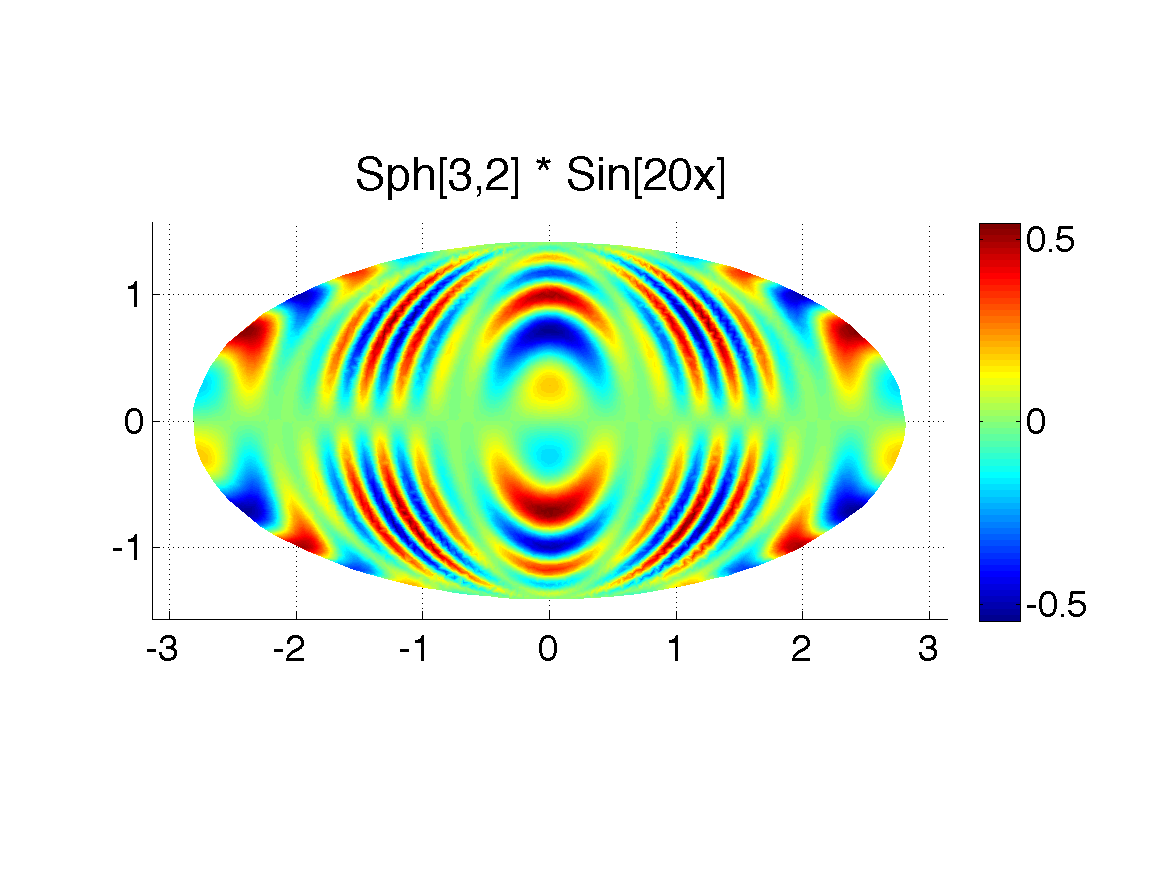
\includegraphics[width=1.0\textwidth]{figures/chapter2/compare_weight_generation/xsfc_vs_xsfc_alt_on_sph32_times_sine_20x/sph32_times_sin20x.pdf}
	\caption{Manufactured test function: \\  $f(\vx) = Y_{3}^{2}(\vx)\sin(20x)$.  }
	\end{subfigure}
	\begin{subfigure}[b]{0.425\textwidth}
	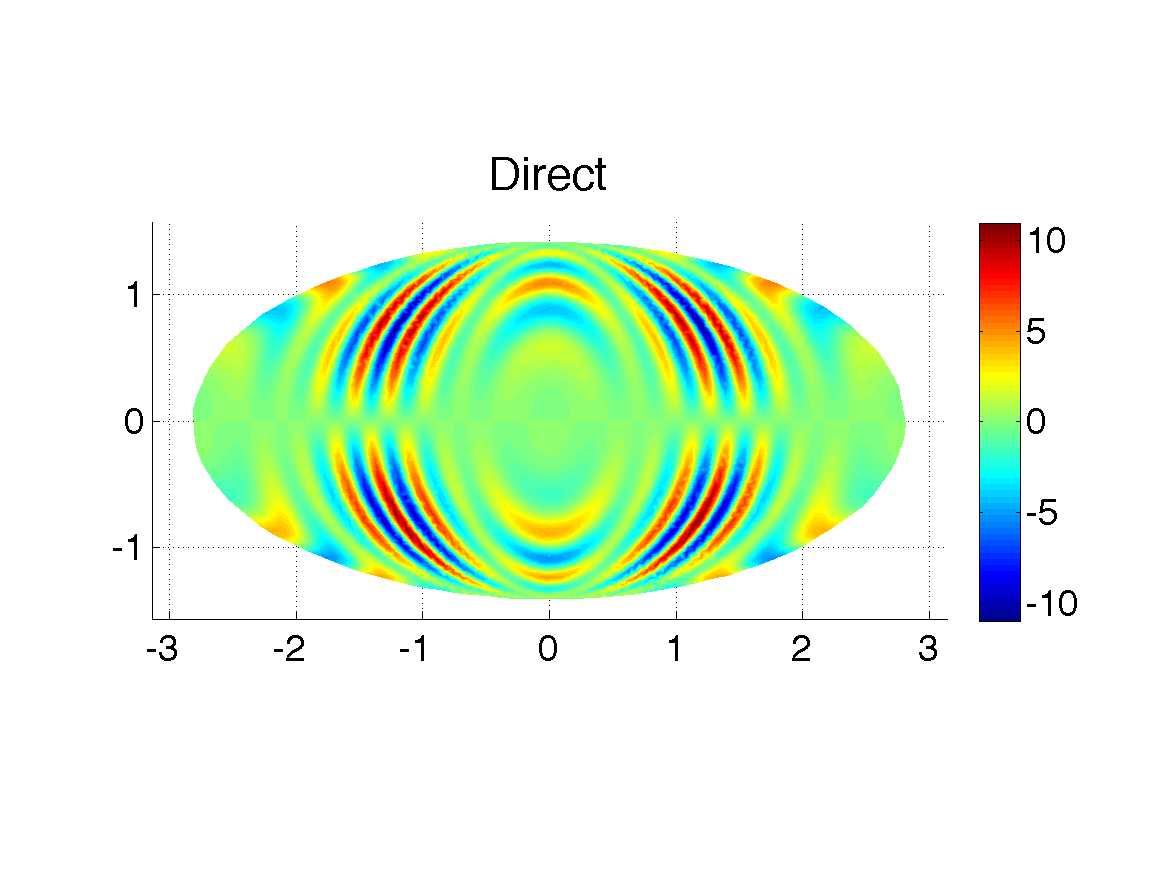
\includegraphics[width=1.0\textwidth]{figures/chapter2/compare_weight_generation/xsfc_vs_xsfc_alt_on_sph32_times_sine_20x/pdx_sph32_times_sin20x.pdf}
	\caption{$x$-component of the projected gradient: $\mathbf{p}_{x} \cdot \nabla f(\vx)$.  }
	\end{subfigure}
	
	\begin{subfigure}[b]{0.425\textwidth}
	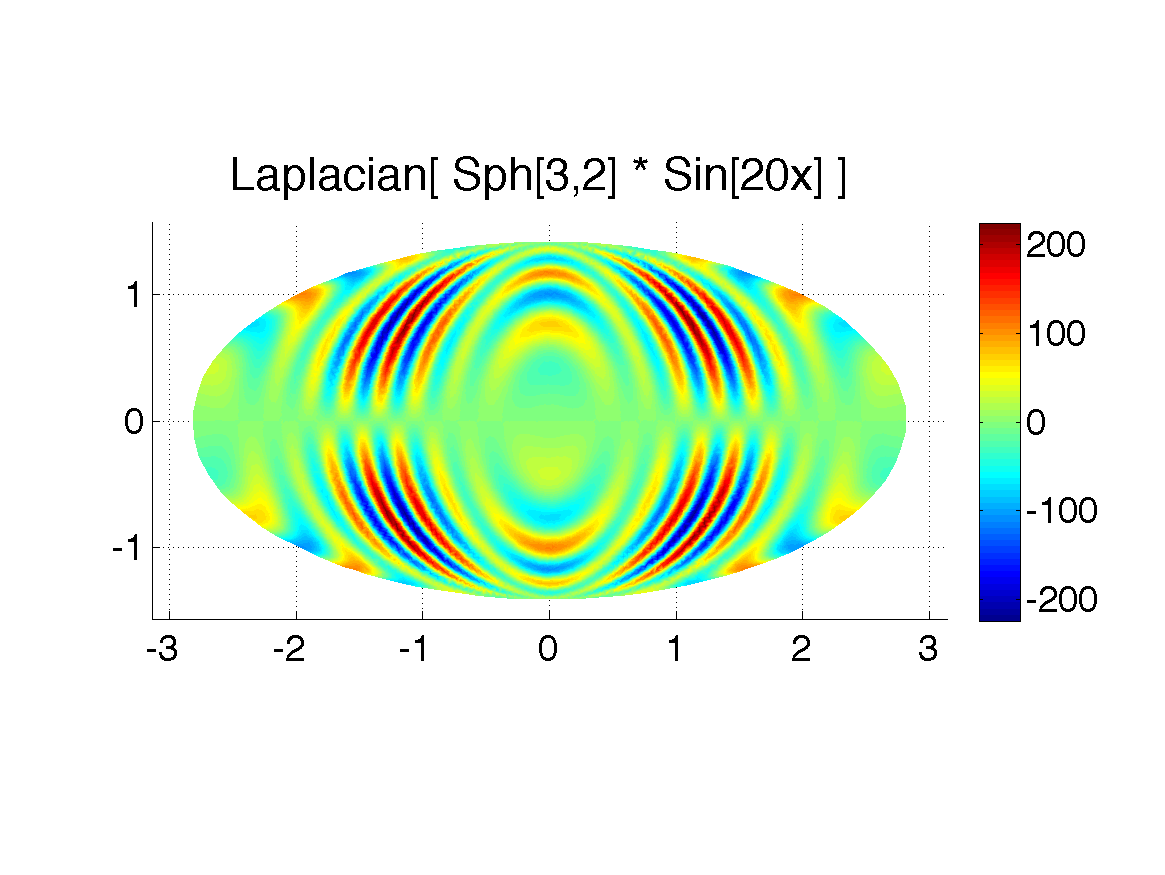
\includegraphics[width=1.0\textwidth]{figures/chapter2/compare_weight_generation/lsfc_vs_px_grad_dot_px_grad/lsfc_sph32_times_sin20x.pdf}
	\caption{Surface Laplacian: $\LaplaceBeltrami f(\vx)$.  }
	\end{subfigure}
	\caption{Test function and its projected $x$ derivatives. }
\end{figure}


\begin{figure}[htbp]
	\centering
	\begin{subfigure}[b]{0.425\textwidth}
	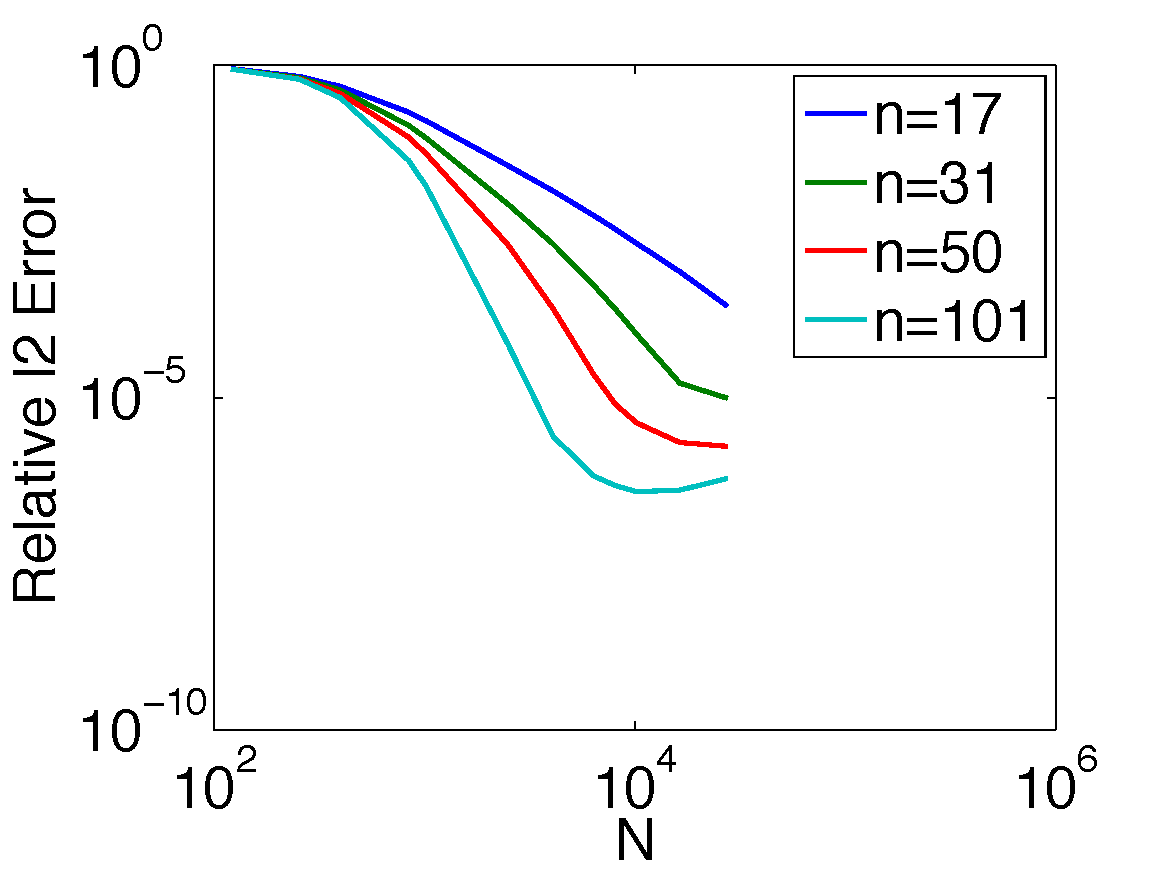
\includegraphics[width=1.0\textwidth]{figures/chapter2/compare_weight_generation/lsfc_vs_px_grad_dot_px_grad/direct_rel_l2_error.pdf}
	\caption{$\LaplaceBeltrami$ of }
		\end{subfigure}
	\begin{subfigure}[b]{0.425\textwidth}
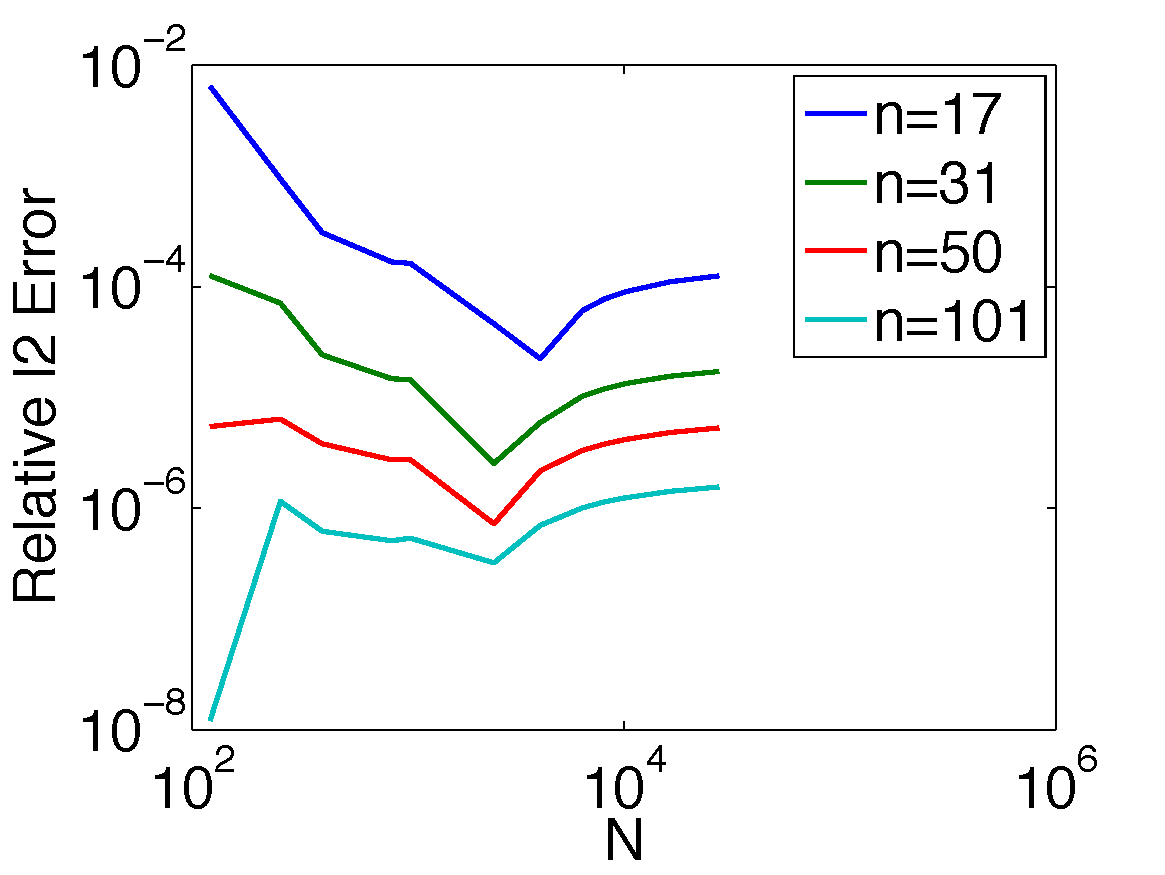
\includegraphics[width=1.0\textwidth]{figures/chapter2/compare_weight_generation/xsfc_vs_xsfc_alt_on_sph32/direct_rel_l2_error.pdf}
	\end{subfigure}
	\begin{subfigure}[b]{0.425\textwidth}
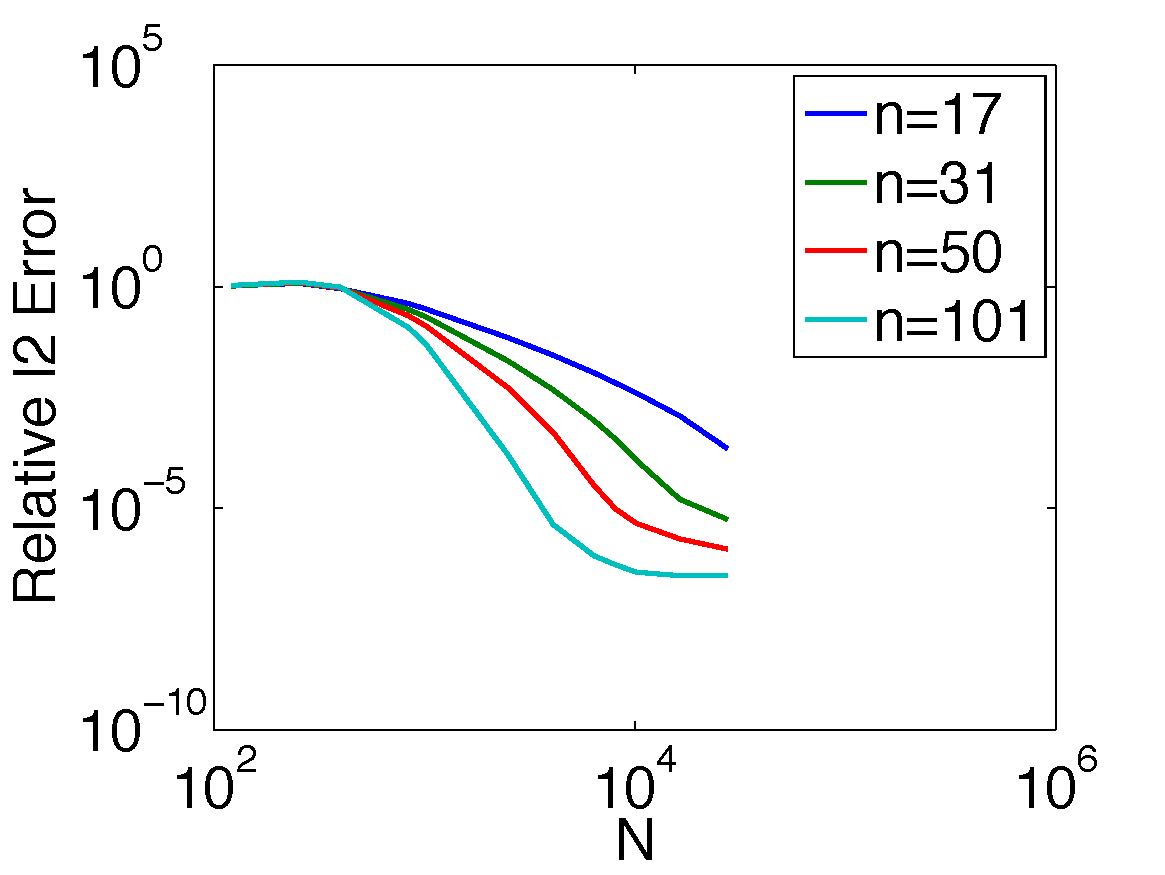
\includegraphics[width=1.0\textwidth]{figures/chapter2/compare_weight_generation/xsfc_vs_xsfc_alt_on_sph32_times_sine_20x/direct_rel_l2_error.pdf}
	\end{subfigure}
	\caption{Relative $\ell_{2}$ error in differentiation.}
\end{figure}


\begin{figure}[htbp]
	\centering
	\begin{subfigure}[b]{0.425\textwidth}
	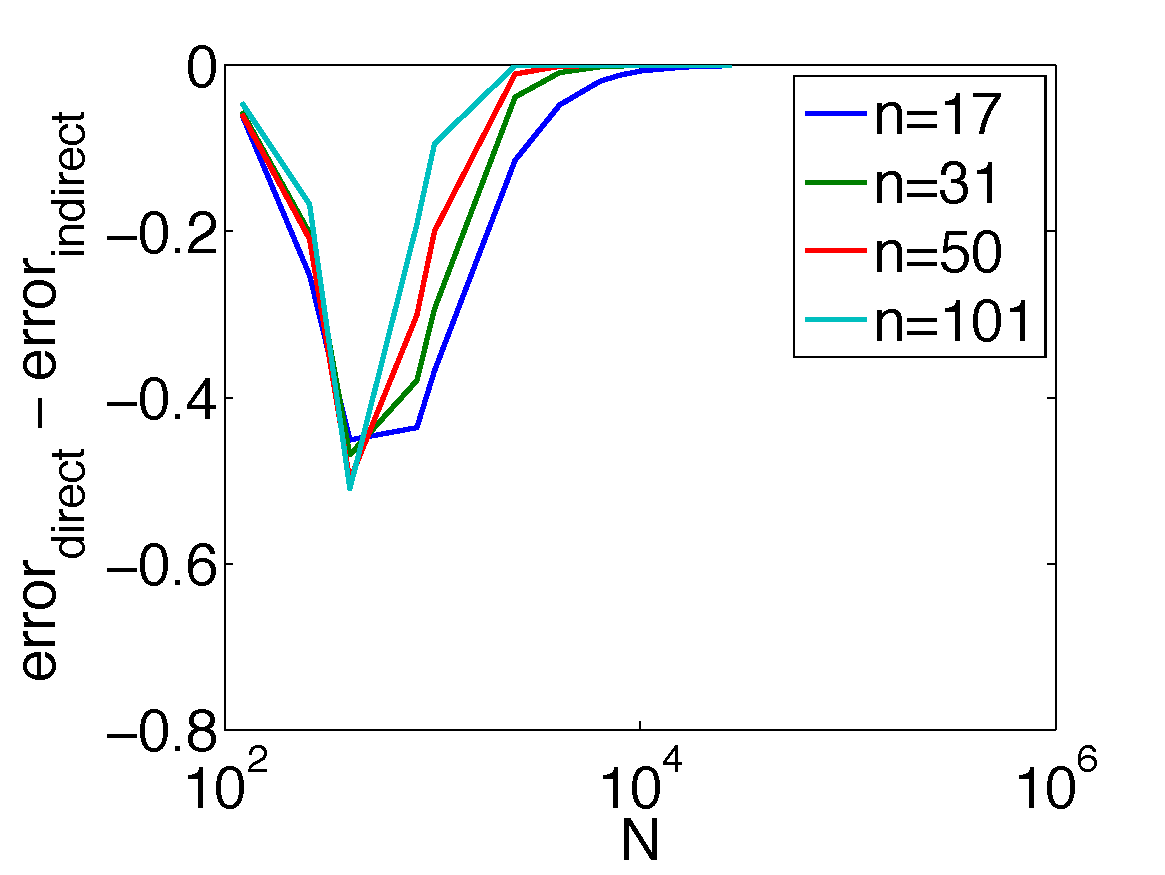
\includegraphics[width=1.0\textwidth]{figures/chapter2/compare_weight_generation/lsfc_vs_px_grad_dot_px_grad/diff_of_rel_l2_errors.pdf}
	\end{subfigure}
	\begin{subfigure}[b]{0.425\textwidth}
	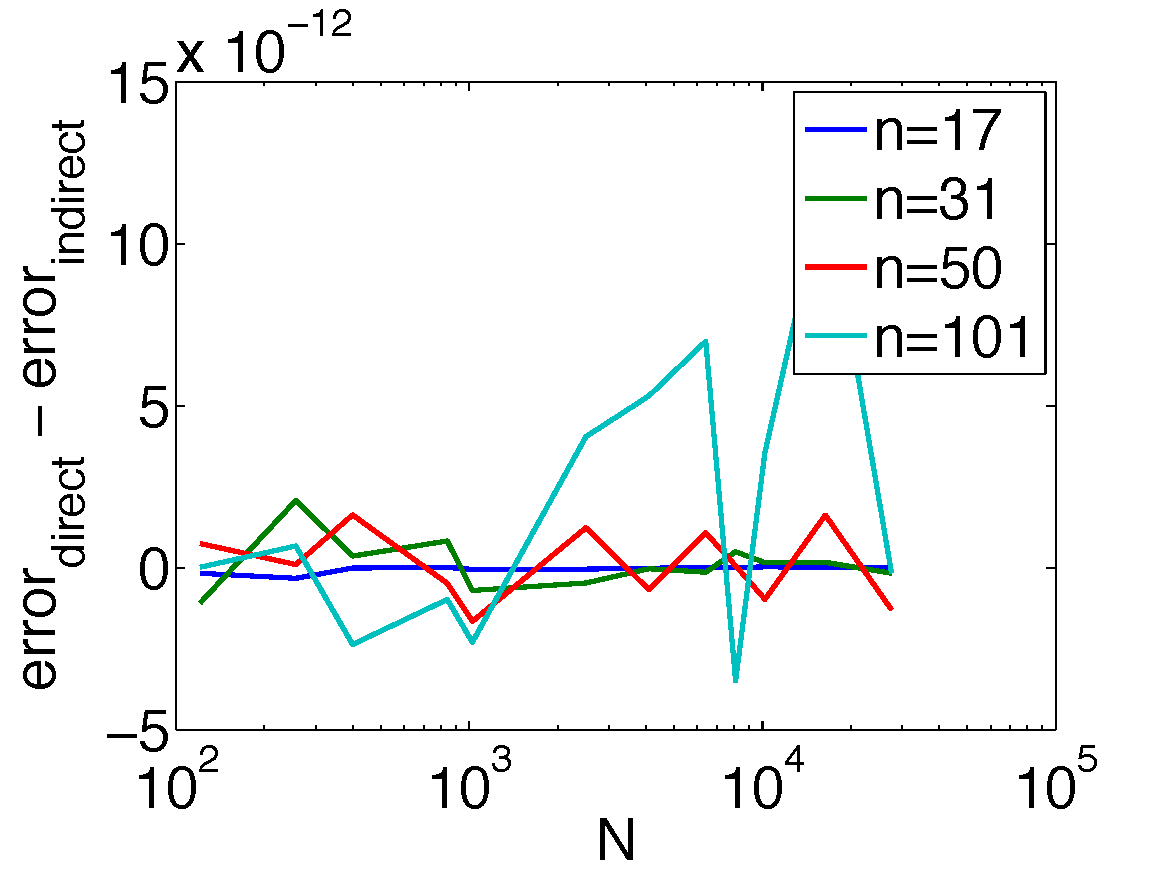
\includegraphics[width=1.0\textwidth]{figures/chapter2/compare_weight_generation/xsfc_vs_xsfc_alt_on_sph32/diff_of_rel_l2_errors.pdf}
	\end{subfigure}
	\begin{subfigure}[b]{0.425\textwidth}
	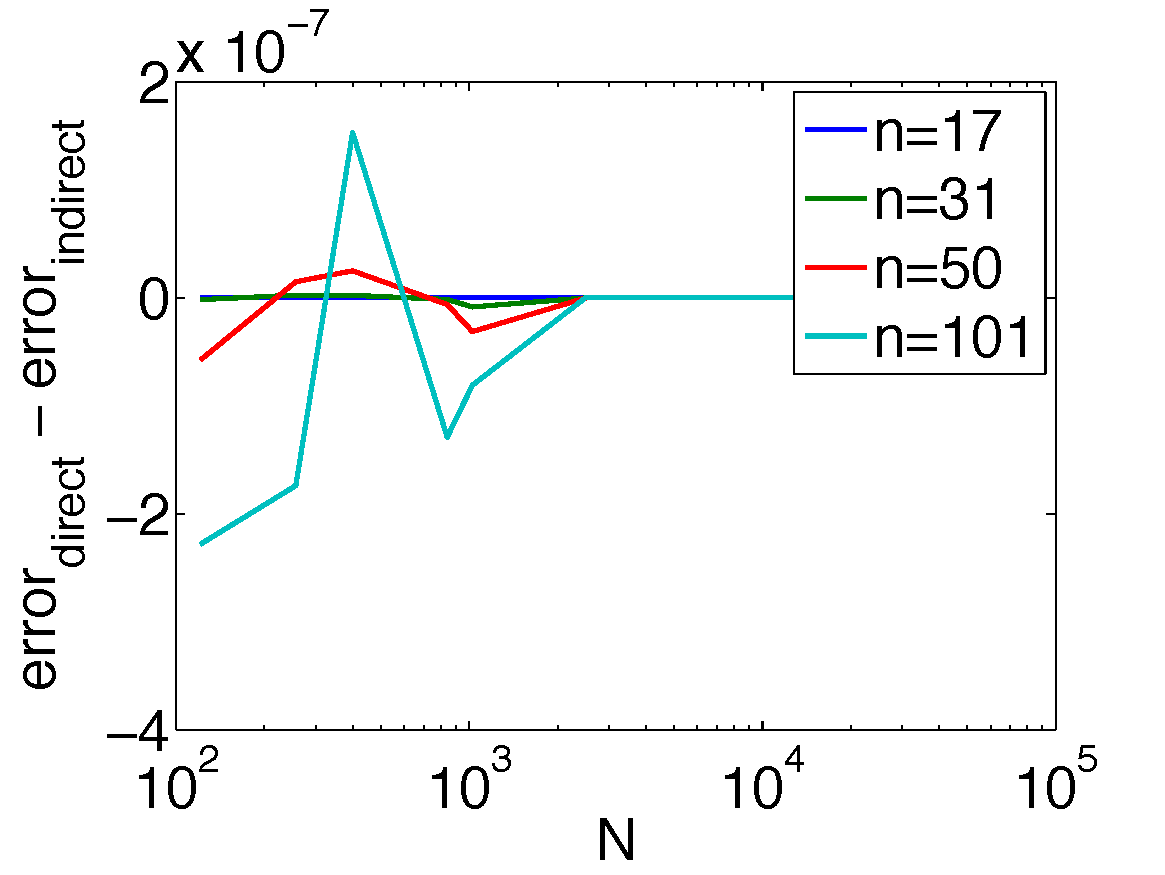
\includegraphics[width=1.0\textwidth]{figures/chapter2/compare_weight_generation/xsfc_vs_xsfc_alt_on_sph32_times_sine_20x/diff_of_rel_l2_errors.pdf}
	\end{subfigure}
	\caption{Signed differences of relative $\ell_{2}$ errors in differentiation between Direct and Indirect weights.}
\end{figure}


\begin{figure}[htbp]
	\centering
	\begin{subfigure}[b]{0.425\textwidth}
	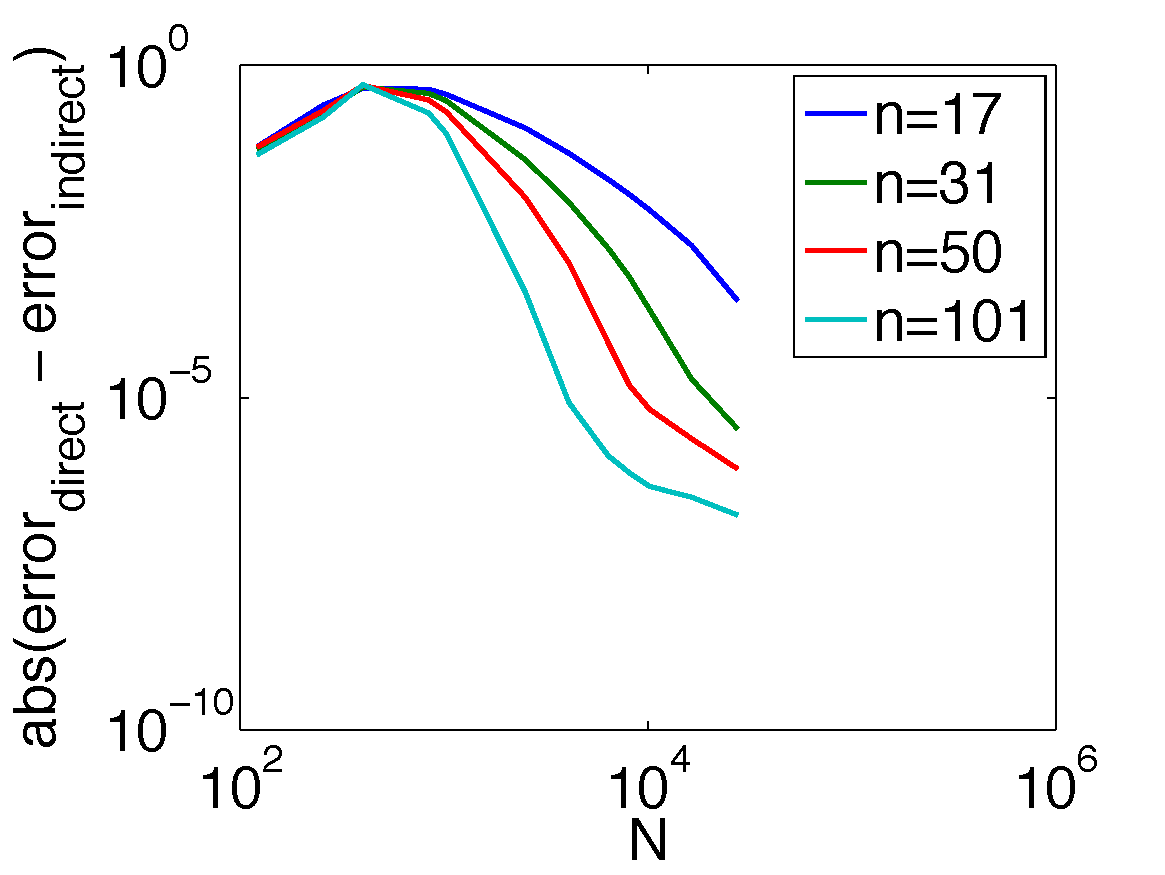
\includegraphics[width=1.0\textwidth]{figures/chapter2/compare_weight_generation/lsfc_vs_px_grad_dot_px_grad/abs_diff_of_rel_l2_errors.pdf}
		\end{subfigure}
	\begin{subfigure}[b]{0.425\textwidth}
	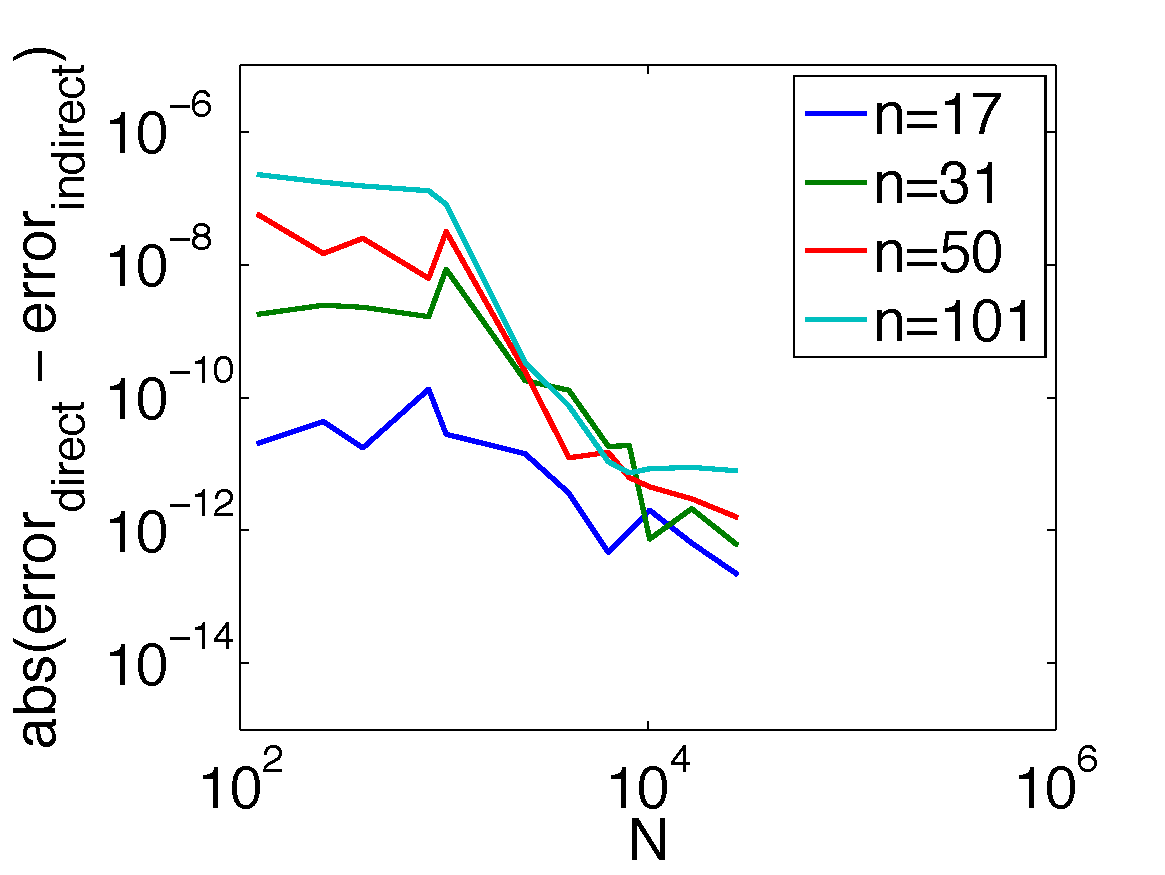
\includegraphics[width=1.0\textwidth]{figures/chapter2/compare_weight_generation/xsfc_vs_xsfc_alt_on_sph32_times_sine_20x/abs_diff_of_rel_l2_errors.pdf}
	\end{subfigure}
		\caption{Absolute differences of relative $\ell_{2}$ errors in differentiation between Direct and Indirect weights.}
\end{figure}

\begin{figure}[htbp]
\centering
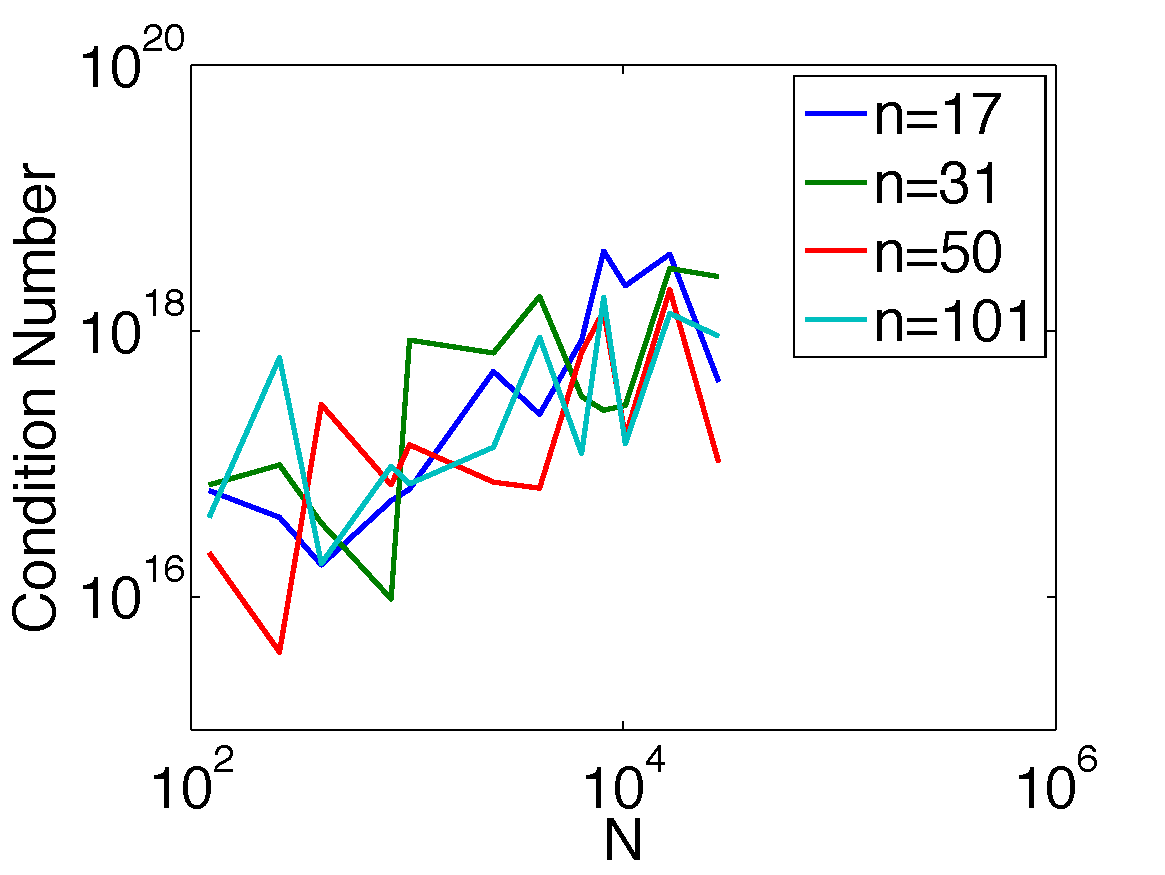
\includegraphics[width=0.425\textwidth]{figures/chapter2/compare_weight_generation/xsfc_vs_xsfc_alt_on_sph32/condest_dm_xsfc.pdf}
\caption{Condition number estimates (condest) of direct $\mathbf{p}_{x}\nabla$ differentiation matrix}
\end{figure}
\section{Conclusions}

Although it is clear the indirect method functions well compared to the direct method, we must consider its usefulness. Typically, weights are computed only as necessary for the PDE. If the PDE is on the sphere, then directly computing the $\mathbf{P}\nabla$ operator would be most efficient for both memory and computation. However, one could imagine a scenario such as a 3-D spherical shell domain with physics on the boundaries that must be constrained to the surface, while the interior requires only an unprojected $\nabla$ operator. In such cases, by simply computing for the $\nabla$ operator, we assemble all necessary operators with minimal loss of accuracy and significant savings ($3Nn$ doubles) in storage. 

\authnote{Plot file size of matrix market file to give an idea of how much memory is saved by cutting out operators} 

With $N=1e6$ nodes and stencil size $n=101$, the matrix market file for weights is approximately 1.6 GB on disk. For a GPU with only 6 GB of global memory space available, it is worthwhile to consider possibilities for memory conservation. 


\authnote{Check to see $\nabla \cdot \nabla$ accuracy for heat equation.} 
